% answers.tex —— 1994 年·上海试点教材理科卷 · 参考答案与详细解析片段
% 由 tools/generate_projects.py 依来源总账自 1994/1994_数学真题_上海试点理_试题.md + 1994/1994_数学真题_上海试点理_解析正文.md + 1994/1994_数学真题_上海试点理_答案要点.md 生成，勿手改（改源 MD 后重跑）


\begin{gktip}
以下按固定 PDF 后附“试题解答及评分标准”整理，统称卷内解答。发布主体、出版者、版次及官方性未核实。题面按原页转录；不以推导反改题面。
\end{gktip}

\begin{answer}
\gksolhead{1}{}

\textbf{题目}：

不等式 \(|x+1|<1\) 的解是\gkblank{}。

\Needspace{4\baselineskip}
\textbf{解析}

由绝对值不等式 \(|x+1|<1\)，得 \(-1<x+1<1\)，所以 \(-2<x<0\)。

\gkanswer{答案：\(-2<x<0\)}

\end{answer}
\begin{answer}
\gksolhead{2}{}

\textbf{题目}：

计算：\(\displaystyle\lim_{x\to-1}\frac{x^2-2x-3}{x+1}=\underline{\qquad}\)。

\Needspace{4\baselineskip}
\textbf{解析}

\Needspace{5\baselineskip}
因式分解并约去 \(x+1\)：
\nopagebreak[4]
\[
\lim_{x\to-1}\frac{x^2-2x-3}{x+1}=\lim_{x\to-1}(x-3)=-4
\]

\gkanswer{答案：\(-4\)}

\end{answer}
\begin{answer}
\gksolhead{3}{}

\textbf{题目}：

以点 \(C(-2,3)\) 为圆心且与 \(y\) 轴相切的圆的方程是\gkblank{}。

\Needspace{4\baselineskip}
\textbf{解析}

圆心 \(C=(-2,3)\) 到 \(y\) 轴距离为 2，即半径为 2，故圆方程为 \((x+2)^2+(y-3)^2=4\)。

\gkanswer{答案：\((x+2)^2+(y-3)^2=4\)}

\end{answer}
\begin{answer}
\gksolhead{4}{}

\textbf{题目}：

方程 \(\log_3(x-1)=\log_9(x+5)\) 的解是\gkblank{}。

\Needspace{4\baselineskip}
\textbf{解析}

由定义域 \(x>1\)，原方程等价于 \(\log_3(x-1)=\frac12\log_3(x+5)\)，故 \((x-1)^2=x+5\)。解得 \(x=4,-1\)，结合定义域取 \(x=4\)。

\gkanswer{答案：\(x=4\)}

\end{answer}
\begin{answer}
\gksolhead{5}{}

\textbf{题目}：

如果复数 \(\dfrac{2+bi}{1-2i}\)（其中 \(i\) 为虚数单位，\(b\) 为实数）的实部和虚部相等，那么 \(b=\underline{\qquad}\)。（据原页转录）

\Needspace{4\baselineskip}
\textbf{解析}

\nopagebreak[4]
\[
\frac{2+bi}{1-2i}=\frac{(2+bi)(1+2i)}5=\frac{2-2b}{5}+\frac{4+b}{5}i
\]
令实部与虚部相等，得 \(2-2b=4+b\)，所以 \(b=-\frac23\)，与卷内答案栏一致。

\gkanswer{答案：\(b=-\dfrac23\)}

\end{answer}
\begin{answer}
\gksolhead{6}{}

\textbf{题目}：

函数 \(y=\sqrt{x^2-1}\ (x\le-1)\) 的反函数是\gkblank{}。

\Needspace{4\baselineskip}
\textbf{解析}

由 \(y=\sqrt{x^2-1}\ (x\le-1)\)，交换变量后有 \(x=\sqrt{y^2-1}\)，故 \(x\ge0\)、\(y^2=x^2+1\)。反函数值取负支，得 \(y=-\sqrt{x^2+1}\ (x\ge0)\)，与卷内答案相同。

\gkanswer{答案：\(y=-\sqrt{x^2+1}\ (x\ge0)\)}

\end{answer}
\begin{answer}
\gksolhead{7}{}

\textbf{题目}：

双曲线 \(\dfrac{y^2}{2}-x^2=1\) 的两个焦点的坐标是\gkblank{}。

\Needspace{4\baselineskip}
\textbf{解析}

双曲线 \(\frac{y^2}{2}-x^2=1\) 的 \(a^2=2,b^2=1\)，所以 \(c^2=a^2+b^2=3\)，焦点为 \((0,\sqrt3)\) 和 \((0,-\sqrt3)\)。

\gkanswer{答案：\((0,\sqrt3)\) 和 \((0,-\sqrt3)\)}

\end{answer}
\begin{answer}
\gksolhead{8}{}

\textbf{题目}：

\(\left(x^3-\dfrac{2}{x^2}\right)^5\) 的展开式中 \(x^5\) 的系数是\gkblank{}。（结果用数值表示）

\Needspace{4\baselineskip}
\textbf{解析}

二项式通项中 \(x\) 的次数为 \(15-5k\)。令 \(15-5k=5\)，得 \(k=2\)，相应系数为 \(\binom52(-2)^2=40\)。

\gkanswer{答案：\(40\)}

\end{answer}
\begin{answer}
\gksolhead{9}{}

\textbf{题目}：

要建造一个长方体形状的仓库，其内部的高为 3 米，长与宽的和为 20 米，那么仓库容积的最大值为\gkblank{}立方米。

\Needspace{4\baselineskip}
\textbf{解析}

设底面长、宽为 \(u,v>0\)，\(u+v=20\)，则 \(uv\le100\)，等号在 \(u=v=10\) 时成立。仓库高为 3，最大容积为 \(3\cdot100=300\) 立方米。

\gkanswer{答案：\(300\)}

\end{answer}
\begin{answer}
\gksolhead{10}{}

\textbf{题目}：

函数 \(\displaystyle y=\frac{\sin 2x+\sin(2x+\pi/3)}{\cos 2x+\cos(2x+\pi/3)}\) 的最小正周期是\gkblank{}。

\Needspace{4\baselineskip}
\textbf{解析}

\Needspace{5\baselineskip}
和差化积得
\nopagebreak[4]
\[
y=\frac{2\sin(2x+\pi/6)\cos(\pi/6)}{2\cos(2x+\pi/6)\cos(\pi/6)}=\tan\left(2x+\frac\pi6\right)
\]
故最小正周期为 \(\frac\pi2\)。

\gkanswer{答案：\(\dfrac\pi2\)}

\end{answer}
\begin{answer}
\gksolhead{11}{}

\textbf{题目}：

当 \(a>1\) 时，函数 \(y=\log_a x\) 和 \(y=(1-a)x\) 的图象只可能是\mbox{（　　）}。

（A）图象 A　（B）图象 B　（C）图象 C　（D）图象 D
\nopagebreak[4]
\begin{center}% 依固定扫描件第 1 页四种函数图象选项转绘；形态示意，不宣称精确比例。
\begin{center}
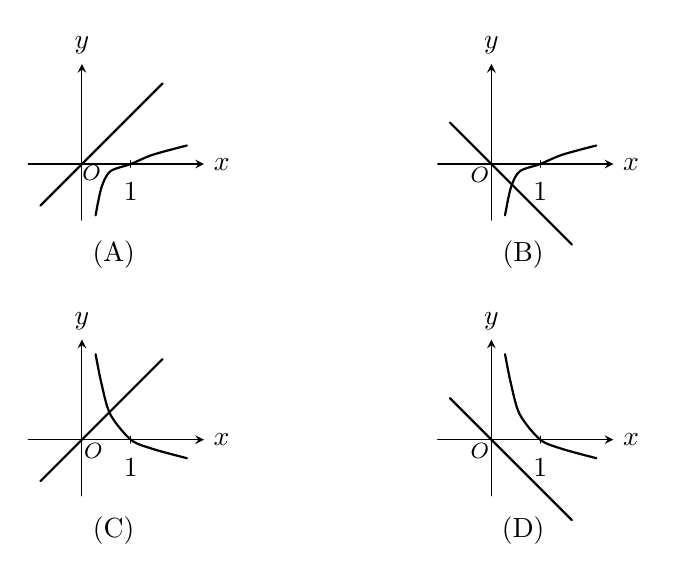
\begin{tikzpicture}[x=0.62cm,y=0.62cm,>=stealth,line cap=round,line join=round]
\foreach \xshift/\yshift/\label/\lineup/\logup/\originplace/\originsep in {
  0/3.5/A/1/1/right/0, 5.2/3.5/B/-1/1/left/0.6,
  0/0/C/1/-1/right/0.6, 5.2/0/D/-1/-1/left/0.6} {
  \begin{scope}[xshift=\xshift cm,yshift=\yshift cm]
    \draw[->] (-1.1,0)--(2.5,0) node[right] {$x$};
    \draw[->] (0,-1.15)--(0,2.05) node[above] {$y$};
    \draw (1,0.07)--(1,-0.07) node[below=2pt] {$1$};
    \node[below \originplace,font=\footnotesize,inner sep=\originsep pt,yshift=-0.4pt] at (0,0) {$O$};
    \ifnum\lineup=1
      \draw[thick] (-0.85,-0.85)--(1.65,1.65);
    \else
      \draw[thick] (-0.85,0.85)--(1.65,-1.65);
    \fi
    \ifnum\logup=1
      \draw[thick] plot[smooth] coordinates {(0.28,-1.05) (0.4,-0.48) (0.58,-0.15) (1,0) (1.45,0.19) (2.15,0.38)};
    \else
      \draw[thick] plot[smooth] coordinates {(0.28,1.75) (0.4,1.15) (0.58,0.52) (1,0) (1.45,-0.19) (2.15,-0.38)};
    \fi
    \node[below] at (0.65,-1.38) {(\label)};
  \end{scope}
}
\end{tikzpicture}
\end{center}
\end{center}
\nopagebreak[4]
\Needspace{4\baselineskip}
\textbf{解析}

\(a>1\) 时，\(y=\log_a x\) 单调递增、过点 \((1,0)\)，直线 \(y=(1-a)x\) 过原点且斜率为负，对应图象 B。

\gkanswer{答案：B}

\end{answer}
\begin{answer}
\gksolhead{12}{}

\textbf{题目}：

如果 \(0<a<1\)，那么下列不等式中正确的是\mbox{（　　）}。

（A）\((1-a)^{1/3}>(1-a)^{1/2}\)　（B）\(\log_{1-a}(1+a)>0\)

（C）\((1-a)^3>(1+a)^2\)　（D）\((1-a)^{1+a}>1\)

\Needspace{4\baselineskip}
\textbf{解析}

因 \(0<1-a<1\)，底数相同且小于 1，指数较小的幂值较大，所以 \((1-a)^{1/3}>(1-a)^{1/2}\)，选 A。

\gkanswer{答案：A}

\end{answer}
\begin{answer}
\gksolhead{13}{}

\textbf{题目}：

已知点 \(P\) 的极坐标为 \((1,\pi)\)，那么过点 \(P\) 且垂直于极轴的直线的极坐标方程是\mbox{（　　）}。

（A）\(\rho=1\)　（B）\(\rho=\cos\theta\)　（C）\(\rho=-\dfrac1{\cos\theta}\)　（D）\(\rho=\dfrac1{\cos\theta}\)

\Needspace{4\baselineskip}
\textbf{解析}

极坐标点 \((1,\pi)\) 对应直角坐标 \((-1,0)\)。过该点且垂直极轴的直线为 \(x=-1\)，即 \(\rho\cos\theta=-1\)，故 \(\rho=-1/\cos\theta\)，选 C。

\gkanswer{答案：C}

\end{answer}
\begin{answer}
\gksolhead{14}{}

\textbf{题目}：

已知 \(a,b\) 是异面直线，直线 \(c\parallel a\)，那么 \(c\) 与 \(b\)\mbox{（　　）}。

（A）一定是异面直线　（B）一定是相交直线　（C）不可能是平行直线　（D）不可能是相交直线

\Needspace{4\baselineskip}
\textbf{解析}

若 \(c\parallel b\)，又 \(c\parallel a\)，则 \(a\parallel b\)，这与 \(a,b\) 异面矛盾。因此 \(c\) 不可能与 \(b\) 平行，选 C。

\gkanswer{答案：C}

\end{answer}
\begin{answer}
\gksolhead{15}{}

\textbf{题目}：

设 \(I\) 是全集，集合 \(P,Q\) 满足 \(P\subset Q\)，则下面结论中错误的是\mbox{（　　）}。

（A）\(P\cup Q=Q\)　（B）\(\overline P\cup Q=I\)　（C）\(P\cap\overline Q=\varnothing\)　（D）\(\overline P\cap\overline Q=\overline P\)

\Needspace{4\baselineskip}
\textbf{解析}

由 \(P\subset Q\)，可得 \(P\cup Q=Q\)、\(\overline P\cup Q=I\)、\(P\cap\overline Q=\varnothing\)。但 \(\overline P\cap\overline Q=\overline Q\)，不必等于 \(\overline P\)，错误项为 D。

\gkanswer{答案：D}

\end{answer}
\begin{answer}
\gksolhead{16}{}

\textbf{题目}：

设复数 \(z=-\dfrac12+\dfrac{\sqrt3}{2}i\)（\(i\) 为虚数单位），则满足等式 \(z^n=z\)，且大于 1 的正整数 \(n\) 中最小的是\mbox{（　　）}。

（A）3　（B）4　（C）6　（D）7

\Needspace{4\baselineskip}
\textbf{解析}

\(z=-\frac12+\frac{\sqrt3}{2}i\) 是非实三次单位根。由 \(z^n=z\) 得 \(z^{n-1}=1\)，故 \(n-1\) 是 3 的正整数倍。大于 1 的最小整数 \(n=4\)，选 B。

\gkanswer{答案：B}

\end{answer}
\begin{answer}
\gksolhead{17}{}

\textbf{题目}：

设 \(a,b\) 是平面 \(\alpha\) 外的任意两条线段，则“\(a,b\) 的长相等”是“\(a,b\) 在平面 \(\alpha\) 内的射影长相等”的\mbox{（　　）}。

（A）非充分条件也非必要条件　（B）充分必要条件　（C）必要条件而非充分条件　（D）充分条件而非必要条件

\Needspace{4\baselineskip}
\textbf{解析}

两线段长度相等不能保证其在平面内的射影长度相等；射影长度相等也不能推出原线段长度相等。因此“长相等”既非充分条件也非必要条件，选 A。

\gkanswer{答案：A}

\end{answer}
\begin{answer}
\gksolhead{18}{}

\textbf{题目}：

9 支足球队中有 5 支亚洲队、4 支非洲队。从中任意抽取两队比赛，则 1 队是亚洲队且 1 队是非洲队的概率是\mbox{（　　）}。

（A）\(\dfrac{\binom51+\binom41}{\binom92}\)　（B）\(\dfrac{\binom41}{\binom92}\)　（C）\(\dfrac{\binom51}{\binom92}\)　（D）\(\dfrac{\binom51\binom41}{\binom92}\)

\Needspace{4\baselineskip}
\textbf{解析}

有利选法是从 5 支亚洲队中取 1 支、从 4 支非洲队中取 1 支，总选法为从 9 支球队中取 2 支，所求概率为 \(\frac{\binom51\binom41}{\binom92}\)，选 D。

\gkanswer{答案：D}

\end{answer}
\begin{answer}
\gksolhead{19}{}

\textbf{题目}：

在直角坐标系 \(xOy\) 中，曲线 \(C\) 的方程是 \(y=\cos x\)。平移坐标系，把原点移到点 \(O\prime\left(\dfrac\pi2,-\dfrac\pi2\right)\)，则在坐标系 \(x\prime O\prime y\prime\) 中曲线 \(C\prime\) 的方程是\mbox{（　　）}。

（A）\(y'=\sin x'+\dfrac\pi2\)　（B）\(y'=-\sin x'+\dfrac\pi2\)　（C）\(y'=\sin x'-\dfrac\pi2\)　（D）\(y'=-\sin x'-\dfrac\pi2\)

\Needspace{4\baselineskip}
\textbf{解析}

新旧坐标关系为 \(x=x\prime+\frac\pi2\)、\(y=y\prime-\frac\pi2\)。代入 \(y=\cos x\)，得 \(y\prime-\frac\pi2=\cos(x\prime+\frac\pi2)=-\sin x\prime\)，所以 \(y\prime=-\sin x\prime+\frac\pi2\)，选 B。

\gkanswer{答案：B}

\end{answer}
\begin{answer}
\gksolhead{20}{}

\textbf{题目}：

某个命题与自然数 \(n\) 有关。如果当 \(n=k\ (k\in\mathbb N)\) 时命题成立，可推得当 \(n=k+1\) 时也成立。现已知 \(n=5\) 时命题不成立，那么可推得\mbox{（　　）}。

（A）\(n=6\) 时不成立　（B）\(n=6\) 时成立　（C）\(n=4\) 时不成立　（D）\(n=4\) 时成立

\Needspace{4\baselineskip}
\textbf{解析}

已知命题满足 \(P(k)\Rightarrow P(k+1)\)，其逆否命题为 \(\neg P(k+1)\Rightarrow\neg P(k)\)。由 \(P(5)\) 不成立，可推出 \(P(4)\) 不成立，选 C。

\gkanswer{答案：C}

\end{answer}
\begin{answer}
\gksolhead{21}{}

\textbf{题目}（12 分）：

已知 \(\sin\alpha=\dfrac35\)，\(\alpha\in(\dfrac\pi2,\pi)\)，\(\tan(\pi-\beta)=\dfrac12\)，求 \(\tan(\alpha-2\beta)\)。

\Needspace{4\baselineskip}
\textbf{解析}

\Needspace{5\baselineskip}
由 \(\sin\alpha=\frac35\)、\(\alpha\in(\frac\pi2,\pi)\)，得 \(\cos\alpha=-\frac45\)、\(\tan\alpha=-\frac34\)。又 \(\tan(\pi-\beta)=\frac12\)，所以 \(\tan\beta=-\frac12\)，\(\tan2\beta=-\frac43\)。于是
\nopagebreak[4]
\[
\tan(\alpha-2\beta)=\frac{-\frac34+\frac43}{1+(-\frac34)(-\frac43)}=\frac7{24}
\]

\gkanswer{答案：\(\tan(\alpha-2\beta)=\dfrac7{24}\)}

\end{answer}
\begin{answer}
\gksolhead{22}{}

\textbf{题目}：

\textbf{（12 分；第（1）小题 7 分，第（2）小题 5 分）}

已知空间三点 \(P(-2,0,2),Q(-1,1,2),R(-3,0,4)\)，设 \(\vec a=\overrightarrow{PQ}\)，\(\vec b=\overrightarrow{PR}\)。

（1） 求 \(\vec a\) 与 \(\vec b\) 的夹角 \(\theta\)（用反三角函数表示）；

（2） 确定实数 \(k\)，使 \(k\vec a+\vec b\) 与 \(k\vec a-2\vec b\) 互相垂直。

\Needspace{4\baselineskip}
\textbf{解析}

\gksubpart{(1) 求夹角}

\(\vec a=(1,1,0)\)，\(\vec b=(-1,0,2)\)，故 \(|\vec a|=\sqrt2\)、\(|\vec b|=\sqrt5\)、\(\vec a\cdot\vec b=-1\)。所以 \(\cos\theta=-\frac{\sqrt{10}}{10}\)，即 \(\theta=\arccos(-\frac{\sqrt{10}}{10})\)。

\gksubpart{(2) 求参数}

\nopagebreak[4]
\[
(k\vec a+\vec b)\cdot(k\vec a-2\vec b)=(k-1)(k+2)+k^2-8=2k^2+k-10
\]
令点积为零，得 \(2k^2+k-10=0\)，所以 \(k=-\frac52\) 或 \(k=2\)。

\gkanswer{答案（1）：\(\theta=\arccos\left(-\dfrac{\sqrt{10}}{10}\right)\)}

\gkanswer{答案（2）：\(k=-\dfrac52\) 或 \(k=2\)}

\end{answer}
\begin{answer}
\gksolhead{23}{}

\textbf{题目}（12 分；两小题各 6 分）：

如图，在梯形 \(ABCD\) 中，\(AD\parallel BC\)，\(\angle ABC=\dfrac\pi2\)，\(AB=a,AD=3a\)，且 \(\angle ADC=\arcsin\dfrac{\sqrt5}{5}\)，又 \(PA\perp\) 平面 \(ABCD\)，\(PA=a\)。求：

（1） 二面角 \(P-CD-A\) 的大小（用反三角函数表示）；

（2） 点 \(A\) 到平面 \(PBC\) 的距离。
\nopagebreak[4]
\begin{center}% 依试点教材理科固定来源 PDF 第 2 页转绘梯形与棱锥的拓扑关系；不表示精确比例。
\begin{center}
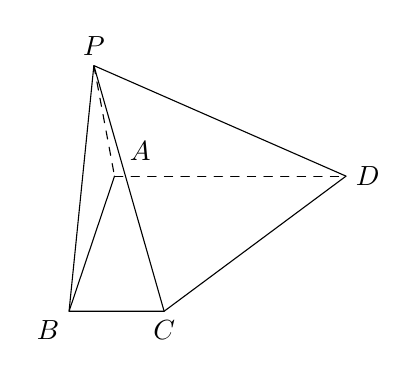
\begin{tikzpicture}[x=1.05cm,y=0.78cm,>=stealth,line cap=round,line join=round]
  \coordinate (B) at (0,0);
  \coordinate (A) at (0.55,2.2);
  \coordinate (C) at (1.15,0);
  \coordinate (D) at (3.35,2.2);
  \coordinate (P) at (0.3,4.0);
  \draw (A)--(B)--(C)--(D);
  \draw[dashed] (A)--(D);
  \draw (P)--(B) (P)--(C) (P)--(D);
  \draw[dashed] (P)--(A);
  \node[above right,xshift=2pt,yshift=2pt] at (A) {$A$};
  \node[below left] at (B) {$B$};
  \node[below] at (C) {$C$};
  \node[right] at (D) {$D$};
  \node[above] at (P) {$P$};
\end{tikzpicture}
\end{center}
\end{center}
\nopagebreak[4]
\Needspace{4\baselineskip}
\textbf{解析}

\gksubpart{(1) 求二面角}

\Needspace{5\baselineskip}
在平面 \(ABCD\) 内过 \(A\) 作 \(AE\perp CD\)，垂足为 \(E\)。因 \(PA\perp\) 平面 \(ABCD\)，由三垂线定理得 \(PE\perp CD\)，故 \(\angle PEA\) 是所求二面角的平面角。直角三角形 \(AED\) 中，
\nopagebreak[4]
\[
AE=AD\sin\angle ADE=3a\cdot\frac{\sqrt5}{5}=\frac{3\sqrt5}{5}a
\]
在直角三角形 \(PAE\) 中，\(\tan\angle PEA=PA/AE=\sqrt5/3\)，所以二面角大小为 \(\arctan(\sqrt5/3)\)。

\gksubpart{(2) 求点到平面的距离}

在平面 \(PAB\) 内过 \(A\) 作 \(AH\perp PB\)。由 \(PA\perp\) 平面 \(ABCD\) 且 \(AB\perp BC\)，得 \(BC\perp\) 平面 \(PAB\)，所以 \(BC\perp AH\)，从而 \(AH\perp\) 平面 \(PBC\)。因此所求距离为 \(AH\)。直角等腰三角形 \(PAB\) 中 \(PA=AB=a\)，故 \(AH=\frac{\sqrt2}{2}a\)。卷内注：若图中点 \(E\) 落在线段 \(CD\) 内，不扣分。

\gkanswer{答案（1）：\(\arctan\dfrac{\sqrt5}{3}\)}

\gkanswer{答案（2）：\(\dfrac{\sqrt2}{2}a\)}

\end{answer}
\begin{answer}
\gksolhead{24}{}

\textbf{题目}（16 分；第（1）小题 6 分，第（2）小题 10 分）：

如图，抛物线 \(y=3x^2\) 和 \(y=-x^2+4tx\) 交于原点 \(O\) 和点 \(A\)。

（1） 当 \(t>0\) 为常数时，求两抛物线所围图形面积；

（2） 过 \(A\) 作抛物线 \(y=-x^2+4tx\) 的切线，该切线与抛物线 \(y=3x^2\) 交于点 \(P\)。当 \(t\) 变化时，求线段 \(AP\) 中点 \(M\) 的轨迹方程，并说明轨迹图形。
\nopagebreak[4]
\begin{center}% 由固定来源示意图按 a=1（或 t=1）重绘；保留两抛物线、公共交点 O/A 与 A 点切线的拓扑关系。
\begin{center}
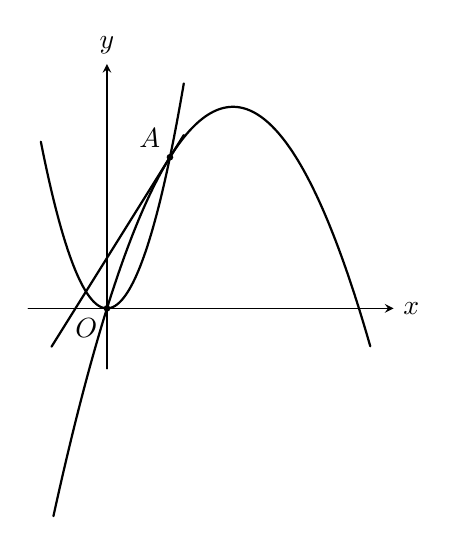
\begin{tikzpicture}[x=0.8cm,y=0.64cm,>=stealth,line cap=round,line join=round]
  \draw[->] (-1.25,0)--(4.55,0) node[right] {$x$};
  \draw[->] (0,-1.2)--(0,4.85) node[above] {$y$};
  \draw[thick,domain=-1.05:1.22,samples=80] plot (\x,{3*\x*\x});
  \draw[thick,domain=-0.85:4.18,samples=120] plot (\x,{-\x*\x+4*\x});
  \draw[thick] (-0.88,-0.76)--(1.22,3.44);
  \fill (0,0) circle (1.2pt);
  \fill (1,3) circle (1.2pt);
  \node[below left] at (0,0) {$O$};
  \node[above left] at (1,3) {$A$};
\end{tikzpicture}
\end{center}
\end{center}
\nopagebreak[4]
\Needspace{4\baselineskip}
\textbf{解析}

\gksubpart{(1) 求面积}

\Needspace{5\baselineskip}
两抛物线交点 \(A=(t,3t^2)\)，所围面积为
\nopagebreak[4]
\[
\int_0^t[(-x^2+4tx)-3x^2]dx=\left(-\frac43x^3+2tx^2\right)_0^t=\frac23t^3
\]

\gksubpart{(2) 求中点轨迹}

曲线 \(y=-x^2+4tx\) 在 \(A=(t,3t^2)\) 处的导数为 \(2t\)，切线为 \(y=2tx+t^2\)。该切线与 \(y=3x^2\) 的另一交点满足 \(3x^2=2tx+t^2\)，解得 \(x=-t/3\)，对应 \(y=t^2/3\)，故 \(P=(-t/3,t^2/3)\)。中点 \(M=(t/3,5t^2/3)\)，消去 \(t\) 得轨迹方程 \(y=15x^2\)，轨迹为抛物线。

\gkanswer{答案（1）：\(\dfrac23t^3\)}

\gkanswer{答案（2）：\(P=\left(-\dfrac t3,\dfrac{t^2}3\right)\)，\(M=\left(\dfrac t3,\dfrac53t^2\right)\)，轨迹为 \(y=15x^2\)}

\end{answer}
\begin{answer}
\gksolhead{25}{}

\textbf{题目}（18 分；第（1）小题 10 分，第（2）小题 8 分）：

直角坐标系中，矩形 \(OPQR\) 顶点按逆时针顺序为 \(O(0,0),P(1,t),Q(1-2t,2+t),R(-2t,2)\)，其中 \(t\in(0,+\infty)\)。

（1） 求矩形在第一象限部分面积 \(S(t)\)；

（2） 确定 \(S(t)\) 的单调区间并证明。

\Needspace{4\baselineskip}
\textbf{解析}

\gksubpart{(1) 求面积函数}

\Needspace{5\baselineskip}
当 \(0<t<\frac12\) 时，边 \(QR\) 与 \(y\) 轴交于 \(K=(0,2t^2+2)\)，矩形第一象限部分减去三角形 \(OKR\)，得
\nopagebreak[4]
\[
S(t)=2(1+t^2)-\frac12(2t^2+2)\cdot2t=2(1-t+t^2-t^3)
\]
当 \(t\ge\frac12\) 时，第一象限部分是三角形 \(OPL\)，其中 \(L=(0,t+1/t)\)，所以 \(S(t)=\frac12(t+1/t)\)。

\gksubpart{(2) 确定单调区间}

\Needspace{5\baselineskip}
当 \(0<t_1<t_2<\frac12\) 时，
\nopagebreak[4]
\[
S(t_1)-S(t_2)=2(t_2-t_1)\left[1-(t_1+t_2)+(t_1^2+t_1t_2+t_2^2)\right]>0
\]
\Needspace{5\baselineskip}
所以 \(S(t)\) 在 \((0,\frac12)\) 上递减。对第二段，
\nopagebreak[4]
\[
S(t_1)-S(t_2)=\frac12(t_1-t_2)\left(1-\frac1{t_1t_2}\right)
\]
由此在 \([\frac12,1]\) 上递减，在 \([1,+\infty)\) 上递增。又 \(S(\frac12)=\frac54\)，且第一段的值小于 \(\frac54\)，所以全域递减区间为 \((0,1]\)，递增区间为 \([1,+\infty)\)。卷内注明：若分别正确写出并证明 \((0,\frac12)\)、\([\frac12,1]\)、\([1,+\infty)\) 三段的单调性，也给分。

\gkanswer{答案（1）：$S(t)=\begin{cases}2(1-t+t^2-t^3),&0<t<\dfrac12,\\[2pt]\dfrac12\left(t+\dfrac1t\right),&t\ge\dfrac12.\end{cases}$}

\gkanswer{答案（2）：递减区间 \((0,1]\)，递增区间 \([1,+\infty)\)}

\end{answer}
\begin{answer}
\gksolhead{26}{}

\textbf{题目}（20 分；第（1）小题 4 分，第（2）小题 8 分，第（3）小题 8 分）：

数列 \(\{a_n\}\) 满足 \(a_1=1,a_2=r\ (r>0)\)，且 \(\{a_na_{n+1}\}\) 是公比为 \(q\ (q>0)\) 的等比数列。设 \(b_n=a_{2n-1}+a_{2n}\)。

（1） 求使 \(a_na_{n+1}+a_{n+1}a_{n+2}>a_{n+2}a_{n+3}\ (n\in\mathbb N)\) 成立的 \(q\) 的范围；

（2） 求 \(b_n\) 及 \(\displaystyle\lim_{n\to\infty}\frac1{S_n}\)，其中 \(S_n=b_1+\cdots+b_n\)；

（3） 设 \(r=2^{19.2}-1\)，\(q=\dfrac12\)，求 \(\left\{\dfrac{\log_2b_{n+1}}{\log_2b_n}\right\}\) 的最大项和最小项。

\Needspace{4\baselineskip}
\textbf{解析}

\gksubpart{(1) 求公比范围}

因 \(a_na_{n+1}\) 成公比为 \(q\) 的等比数列，\(a_{n+1}a_{n+2}=q a_na_{n+1}\)，\(a_{n+2}a_{n+3}=q^2a_na_{n+1}\)。题设不等式等价于 \(1+q>q^2\)。结合 \(q>0\)，得 \(0<q<\frac{1+\sqrt5}{2}\)。

\gksubpart{(2) 求 \(b_n\) 与极限}

\nopagebreak[4]
\[
\frac{b_{n+1}}{b_n}=\frac{a_{2n+1}+a_{2n+2}}{a_{2n-1}+a_{2n}}=q
\]
且 \(b_1=1+r\)，故 \(b_n=(1+r)q^{n-1}\)。于是 \(S_n\) 是首项 \(1+r\)、公比 \(q\) 的等比数列前 \(n\) 项和。若 \(0<q<1\)，\(S_n=(1+r)(1-q^n)/(1-q)\)，所以 \(\lim_{n\to\infty}1/S_n=(1-q)/(1+r)\)。若 \(q=1\)，\(S_n=n(1+r)\)；若 \(q>1\)，\(S_n\to+\infty\)。故 \(q\ge1\) 时该极限为 0。卷内评分注：只写 \(b_n\) 而未说明理由，扣 2 分。

\gksubpart{(3) 求最大项和最小项}

\Needspace{5\baselineskip}
题设 \(r=2^{19.2}-1\)、\(q=1/2\)，故由（2）得 \(b_n=2^{19.2-n+1}=2^{20.2-n}\)，从而
\nopagebreak[4]
\[
c_n=\frac{\log_2b_{n+1}}{\log_2b_n}=\frac{20.2-(n+1)}{20.2-n}=1+\frac1{n-20.2}
\]
当整数 \(n\ge21\) 时，\(c_n\) 随 \(n\) 增大而减小，最大值为 \(c_{21}=2.25\)；当 \(n\le20\) 时也随 \(n\) 增大而减小，最小值为 \(c_{20}=-4\)。题面指数 \(19.2\) 与卷内化简中出现的 \(20.2\) 相容，因为 \(\log_2b_n=19.2-(n-1)=20.2-n\)。

\gkanswer{答案（1）：\(0<q<\dfrac{1+\sqrt5}{2}\)}

\gkanswer{答案（2）：$b_n=(1+r)q^{n-1}$，$\displaystyle\lim_{n\to\infty}\frac1{S_n}=\begin{cases}\dfrac{1-q}{1+r},&0<q<1,\\[2pt]0,&q\ge1.\end{cases}$}

\gkanswer{答案（3）：最大项为 \(2.25\)，最小项为 \(-4\)}

\end{answer}